\section{Full Fixed-Mask Matrix}
\label{supp:fixed-mask}

The following tables retain all fixed-mask deterministic evaluations by dataset. Only historical inputs are masked; targets are unchanged.

\begin{table}[ht]\centering\caption{Full ETTh1 fixed-mask matrix.}\label{tab:supp-etth1}\scriptsize\resizebox{\linewidth}{!}{\begin{tabular}{@{}lrrrr@{}}
\toprule
Mask & Rate & MSE & MAE & RMSE \\
\midrule
Block & 0.10 & 0.388818 & 0.416915 & 0.623552 \\
Block & 0.30 & 0.423837 & 0.451188 & 0.651027 \\
Block & 0.50 & 0.486504 & 0.501242 & 0.697498 \\
Block & 0.70 & 0.591697 & 0.571655 & 0.769219 \\
Channel & 0.10 & 0.479410 & 0.455063 & 0.692394 \\
Channel & 0.30 & 0.583704 & 0.511084 & 0.764006 \\
Channel & 0.50 & 0.798862 & 0.627325 & 0.893791 \\
Channel & 0.70 & 0.900947 & 0.683061 & 0.949182 \\
Mixed & 0.10 & 0.486209 & 0.464128 & 0.697287 \\
Mixed & 0.30 & 0.495055 & 0.473908 & 0.703601 \\
Mixed & 0.50 & 0.553485 & 0.525226 & 0.743966 \\
Mixed & 0.70 & 0.715806 & 0.617339 & 0.846053 \\
Random & 0.10 & 0.378811 & 0.408069 & 0.615476 \\
Random & 0.30 & 0.425394 & 0.450336 & 0.652223 \\
Random & 0.50 & 0.525856 & 0.523115 & 0.725160 \\
Random & 0.70 & 0.688520 & 0.617690 & 0.829771 \\
\bottomrule
\end{tabular}
}\end{table}
\begin{table}[ht]\centering\caption{Full Weather fixed-mask matrix.}\label{tab:supp-weather}\scriptsize\resizebox{\linewidth}{!}{\begin{tabular}{@{}lrrrr@{}}
\toprule
Mask & Rate & MSE & MAE & RMSE \\
\midrule
Block & 0.10 & 0.158302 & 0.218956 & 0.397872 \\
Block & 0.30 & 0.180420 & 0.245178 & 0.424759 \\
Block & 0.50 & 0.210474 & 0.277453 & 0.458774 \\
Block & 0.70 & 0.254572 & 0.322297 & 0.504551 \\
Channel & 0.10 & 0.191289 & 0.238851 & 0.437366 \\
Channel & 0.30 & 0.284471 & 0.316355 & 0.533358 \\
Channel & 0.50 & 0.377902 & 0.393866 & 0.614738 \\
Channel & 0.70 & 0.495709 & 0.490618 & 0.704066 \\
Mixed & 0.10 & 0.175815 & 0.230739 & 0.419303 \\
Mixed & 0.30 & 0.224939 & 0.281431 & 0.474278 \\
Mixed & 0.50 & 0.306930 & 0.357264 & 0.554012 \\
Mixed & 0.70 & 0.400193 & 0.440502 & 0.632608 \\
Random & 0.10 & 0.169631 & 0.232543 & 0.411863 \\
Random & 0.30 & 0.240810 & 0.309629 & 0.490724 \\
Random & 0.50 & 0.331313 & 0.391138 & 0.575598 \\
Random & 0.70 & 0.434543 & 0.474367 & 0.659199 \\
\bottomrule
\end{tabular}
}\end{table}
\begin{table}[ht]\centering\caption{Full Electricity fixed-mask matrix.}\label{tab:supp-electricity}\scriptsize\resizebox{\linewidth}{!}{\begin{tabular}{@{}lrrrr@{}}
\toprule
Mask & Rate & MSE & MAE & RMSE \\
\midrule
Block & 0.10 & 0.143247 & 0.243795 & 0.378480 \\
Block & 0.30 & 0.184630 & 0.289155 & 0.429686 \\
Block & 0.50 & 0.270835 & 0.369677 & 0.520418 \\
Block & 0.70 & 0.464169 & 0.520260 & 0.681300 \\
Channel & 0.10 & 0.213972 & 0.281108 & 0.462571 \\
Channel & 0.30 & 0.391038 & 0.403166 & 0.625331 \\
Channel & 0.50 & 0.569116 & 0.525639 & 0.754398 \\
Channel & 0.70 & 0.748916 & 0.649662 & 0.865399 \\
Mixed & 0.10 & 0.165759 & 0.254616 & 0.407135 \\
Mixed & 0.30 & 0.246785 & 0.325159 & 0.496775 \\
Mixed & 0.50 & 0.375182 & 0.437690 & 0.612521 \\
Mixed & 0.70 & 0.588662 & 0.596810 & 0.767243 \\
Random & 0.10 & 0.138429 & 0.242728 & 0.372060 \\
Random & 0.30 & 0.200572 & 0.318891 & 0.447853 \\
Random & 0.50 & 0.325732 & 0.432183 & 0.570729 \\
Random & 0.70 & 0.546080 & 0.584678 & 0.738972 \\
\bottomrule
\end{tabular}
}\end{table}

\section{TimePerceiver Seed-Level Summaries}
\label{supp:timeperceiver-seeds}
The four probability-head seeds are 2021, 2022, 2023, and 2025 on fixed official backbone checkpoints. The panels summarize the dataset-level means and variability; the main manuscript preserves all paired NLL deltas.
\begin{figure}[ht]\centering
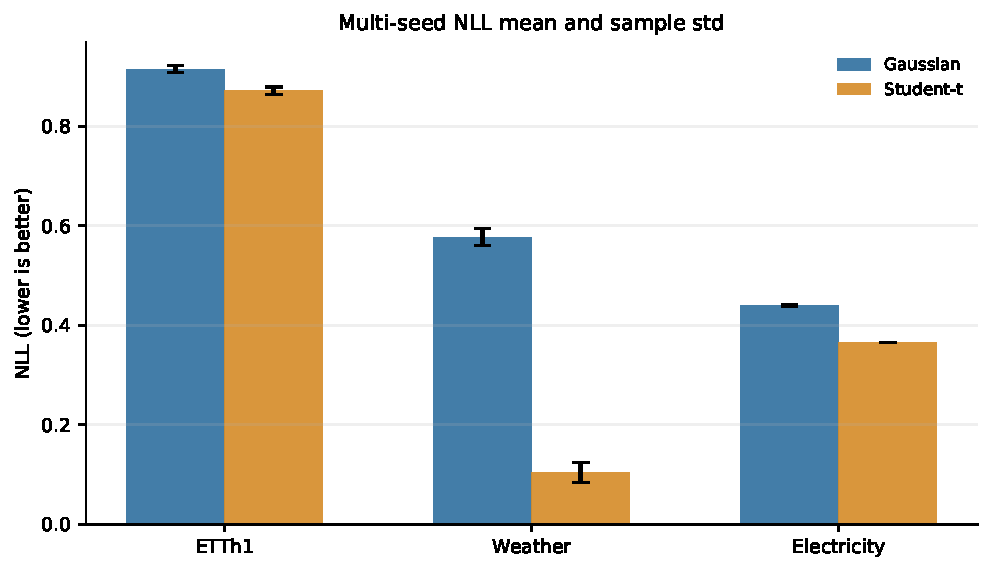
\includegraphics[width=0.32\linewidth]{fig3a_multiseed_nll.pdf}
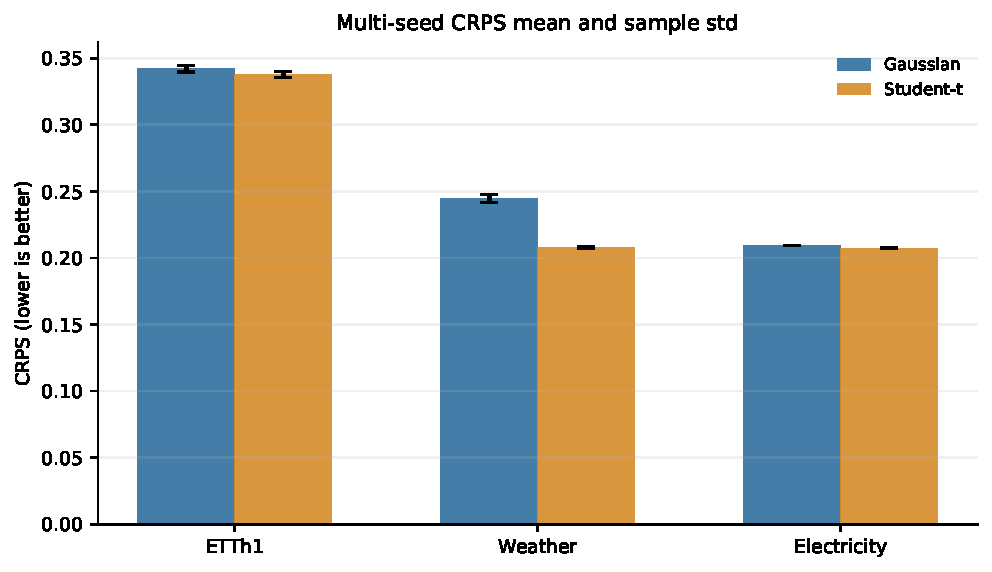
\includegraphics[width=0.32\linewidth]{fig3b_multiseed_crps.pdf}
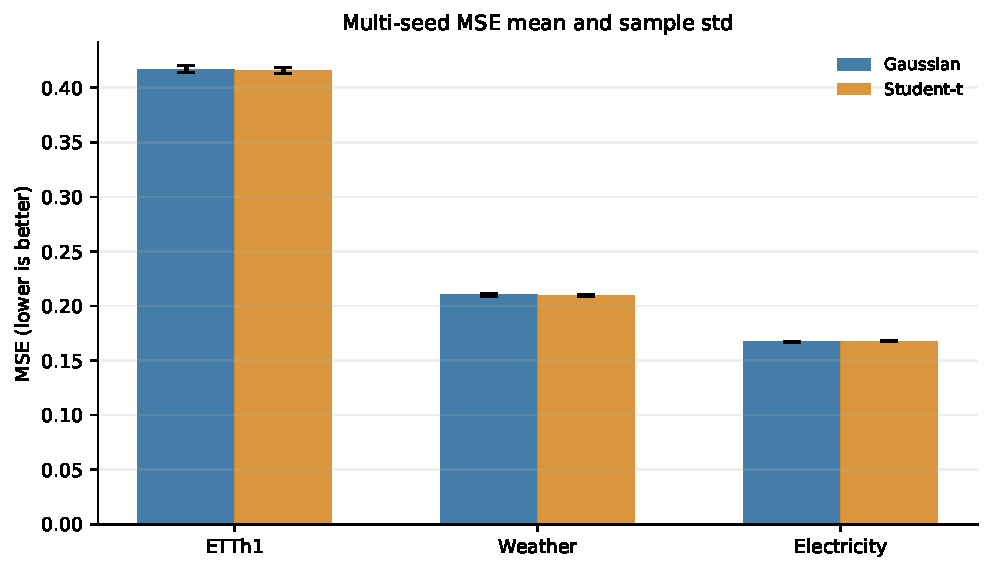
\includegraphics[width=0.32\linewidth]{fig3c_multiseed_mse.pdf}
\caption{TimePerceiver probability-head seed summaries for NLL, CRPS, and MSE.}\label{fig:supp-multiseed}
\end{figure}
\begin{table}[ht]\centering\caption{ETTh1 paired results across additional missing-history conditions. Negative deltas favor fixed \StudentT{}.}\label{tab:supp-etth1-conditions}\scriptsize\resizebox{\linewidth}{!}{\begin{tabular}{@{}lrrrrrr@{}}
\toprule
Condition & $\Delta$NLL & $\Delta$CRPS & $\Delta$MSE & NLL win & CRPS NI & Point NI \\
\midrule
Random 0.1 & -0.078025 & -0.006113 & -0.002231 & Yes & Yes & Yes \\
Random 0.3 & -0.041381 & -0.003864 & -0.001155 & Yes & Yes & Yes \\
Random 0.5 & -0.013720 & 0.000656 & 0.007100 & Yes & No & No \\
Block 0.3 & -0.061086 & -0.007738 & -0.004834 & Yes & Yes & Yes \\
Channel 0.3 & -0.071504 & -0.004849 & 0.001022 & Yes & Yes & Yes \\
Mixed 0.3 & -0.070665 & -0.003286 & 0.001169 & Yes & Yes & Yes \\
\bottomrule
\end{tabular}
}\end{table}
